%===============================================================================
% LaTeX sjabloon voor de bachelorproef toegepaste informatica aan HOGENT
% Meer info op https://github.com/HoGentTIN/bachproef-latex-sjabloon
%===============================================================================

\documentclass{bachproef-tin}

\usepackage{hogent-thesis-titlepage} % Titelpagina conform aan HOGENT huisstijl
\usepackage{subfig}
\usepackage[cache=false]{minted}
\usemintedstyle{vs}

%%---------- Documenteigenschappen ---------------------------------------------
% TODO: Vul dit aan met je eigen info:

% De titel van het rapport/bachelorproef
\title{End to End Testing Framework voor de Nieuwe Front-End van Colruyt Group's Checkoutsysteem: Vergelijkende Studie \& Proof of Concept}

% Je eigen naam
\author{Pieter-Jan Van Damme}

% De naam van je promotor (lector van de opleiding)
\promotor{Antonia Pierreux}

% De naam van je co-promotor. Als je promotor ook je opdrachtgever is en je
% dus ook inhoudelijk begeleidt (en enkel dan!), mag je dit leeg laten.
\copromotor{Koen Stockman}

% Indien je bachelorproef in opdracht van/in samenwerking met een bedrijf of
% externe organisatie geschreven is, geef je hier de naam. Zoniet laat je dit
% zoals het is.
\instelling{Colruyt Group Services nv}

% Academiejaar
\academiejaar{2019-2020}

% Examenperiode
%  - 1e semester = 1e examenperiode => 1
%  - 2e semester = 2e examenperiode => 2
%  - tweede zit  = 3e examenperiode => 3
\examenperiode{2}

%===============================================================================
% Inhoud document
%===============================================================================

\begin{document}

%---------- Taalselectie -------------------------------------------------------
% Als je je bachelorproef in het Engels schrijft, haal dan onderstaande regel
% uit commentaar. Let op: de tekst op de voorkaft blijft in het Nederlands, en
% dat is ook de bedoeling!

\selectlanguage{dutch}

%---------- Titelblad ----------------------------------------------------------
\inserttitlepage

%---------- Samenvatting, voorwoord --------------------------------------------
\usechapterimagefalse
%%=============================================================================
%% Voorwoord
%%=============================================================================

\chapter*{\IfLanguageName{dutch}{Woord vooraf}{Preface}}
\label{ch:voorwoord}

%% TODO:
%% Het voorwoord is het enige deel van de bachelorproef waar je vanuit je
%% eigen standpunt (``ik-vorm'') mag schrijven. Je kan hier bv. motiveren
%% waarom jij het onderwerp wil bespreken.
%% Vergeet ook niet te bedanken wie je geholpen/gesteund/... heeft

Vier en een half jaar geleden schreef ik me in voor de opleiding bachelor in de toegepaste informatica in afstandsonderwijs. Ik was een iets jongere man en was vastberaden de koers van mijn leven om te slaan naar een andere windrichting. Het behalen van dit diploma — in combinatie met een fulltime job — zal één van mijn belangrijkste verwezenlijkingen zijn.

De reis is niet altijd verlopen zoals verwacht. De gezondheidscrisis die de wereld momenteel in zijn grip heeft, stond geenzins op de planning. Hetzelfde geldt voor mijn aanwerving bij Colruyt Group in het voorjaar van 2018. Hoewel mijn opleiding nog niet afgerond was, gaf de firma mij het vertrouwen om mijn carrière als ICT-professional te beginnen in een rol als functioneel analist.

Het onderwerp van mijn bachelorproef — een vergelijkende studie van kandidaat testing frameworks voor het nieuwe front-end systeem van Colruyt Group's kassasysteem — is niet toevallig gekozen. Als analist binnen de afdeling ``point of sale \& payment'' houdt ik me voornamelijk bezig met projecten met impact op het checkoutsysteem. Deze bachelorproef ligt dus in het verlengde van mijn specialisatie en laat me toe op een andere manier impact te hebben.

Ik stond er echter niet alleen voor. Ik wil in de eerste plaats Antonia Pierreux bedanken voor haar begeleiding tijdens de bachelorproef. Haar pragmatische en optimistische houding hebben me zeker geïnspireerd om deze scriptie tot een goed einde te brengen.

Koen Stockman, mijn co-promotor en applicatiemanager binnen mijn afdeling, Kenneth Aerens, onze Angular coach, en Thanuja Mudiyala, test lead voor Colruyt India, wil ik evenzeer bedanken. Gedurende mijn 2 jaar als analist bij Colruyt Group heb ik altijd graag met hen samengewerkt als collega's. Ook tijdens het uitwerken van deze bachelorproef hebben ze mij ondersteund met veel expertise en aanmoediging.

Ik wil ook Greet Dolvelde, sr. analist van onze afdeling, en Luc Devits, mijn directe chef, bedanken om mij de ademruimte die ik nodig had om mijn opleiding af te ronden te gunnen.

Vele anderen  hebben mij aangemoedigd tijdens mijn studie. Deze studie was een herculische taak die meer offers vroeg dan ik initieel had verwacht. Zonder de vele andere mensen in mijn leven — familie, vrienden en collega's — had ik dit nooit kunnen bereiken. Bij deze: dank jullie allemaal!

Ten slotte bedank ik ook u, de lezer, en hoop ik dat mijn werk u mag informeren en inspireren.

\begin{flushright}
Pieter-Jan Van Damme\linebreak
Lede, 20/08/2020
\end{flushright}
%%=============================================================================
%% Samenvatting
%%=============================================================================

% TODO: De "abstract" of samenvatting is een kernachtige (~ 1 blz. voor een
% thesis) synthese van het document.
%
% Deze aspecten moeten zeker aan bod komen:
% - Context: waarom is dit werk belangrijk?
% - Nood: waarom moest dit onderzocht worden?
% - Taak: wat heb je precies gedaan?
% - Object: wat staat in dit document geschreven?
% - Resultaat: wat was het resultaat?
% - Conclusie: wat is/zijn de belangrijkste conclusie(s)?
% - Perspectief: blijven er nog vragen open die in de toekomst nog kunnen
%    onderzocht worden? Wat is een mogelijk vervolg voor jouw onderzoek?
%
% LET OP! Een samenvatting is GEEN voorwoord!


%%---------- Samenvatting -----------------------------------------------------
% De samenvatting in de hoofdtaal van het document

\chapter*{\IfLanguageName{dutch}{Samenvatting}{Abstract}}

Bij elk softwareproject is de keuze voor het gepaste framework één van de belangrijkste factoren in het succes ervan. Dit geldt evenzeer voor test automatisatieprojecten. Colruyt Group ontwikkelt momenteel een nieuwe Angular front-end applicatie voor hun checkoutsysteem en wil ook investeren in test automatisatie. Zij beschikken reeds over een end-to-end testing framework — UFT — maar ondervinden een aantal belangrijke nadelen. De firma overweegt twee andere kandidaten — Protractor en Cypress — en wil advies omtrent het geschikte framework voor hun situatie. Om dit advies te kunnen leveren werden de kandidaat frameworks onderworpen aan een requirementsanalyse enerzijds, en een praktijktest anderzijds. In deze praktijktest werden 5 dezelfde testen in UFT en Cypress uitgevoerd en werd hun performantie gemonitord. De test voor Protractor kon omwille van tijdsgebrek helaas niet gerealizeerd worden. Hieruit bleek dat Cypress de meest geschikte kandidaat is, rekening houdende met alle factoren. Desondanks is er nog ruimte voor verbetering: idealiter zouden alle praktijktesten herhaald worden met een prototype van de applicatie, een gemockte backend en éénzelfde simulator voor de randapparaten. Desondanks geeft dit onderzoek reeds een goed beeld over hoe de frameworks zich tegenover elkaar verhouden. Het advies aan Colruyt Group is dus om voor Cypress te kiezen, met Protractor als tweede keuze.


%---------- Inhoudstafel -------------------------------------------------------
\pagestyle{empty} % Geen hoofding
\tableofcontents  % Voeg de inhoudstafel toe
\cleardoublepage  % Zorg dat volgende hoofstuk op een oneven pagina begint
\pagestyle{fancy} % Zet hoofding opnieuw aan

%---------- Lijst figuren, afkortingen, ... ------------------------------------

% Indien gewenst kan je hier een lijst van figuren/tabellen opgeven. Geef in
% dat geval je figuren/tabellen altijd een korte beschrijving:
%
%  \caption[korte beschrijving]{uitgebreide beschrijving}
%
% De korte beschrijving wordt gebruikt voor deze lijst, de uitgebreide staat bij
% de figuur of tabel zelf.

\listoffigures
\listoftables

% Als je een lijst van afkortingen of termen wil toevoegen, dan hoort die
% hier thuis. Gebruik bijvoorbeeld de ``glossaries'' package.
% https://www.overleaf.com/learn/latex/Glossaries

%---------- Kern ---------------------------------------------------------------

% De eerste hoofdstukken van een bachelorproef zijn meestal een inleiding op
% het onderwerp, literatuurstudie en verantwoording methodologie.
% Aarzel niet om een meer beschrijvende titel aan deze hoofstukken te geven of
% om bijvoorbeeld de inleiding en/of stand van zaken over meerdere hoofdstukken
% te verspreiden!

%%=============================================================================
%% Inleiding
%%=============================================================================

\chapter{\IfLanguageName{dutch}{Inleiding}{Introduction}}
\label{ch:inleiding}

Softwareontwikkeling is een relatief jonge industrie, maar ook één die aan een ijltempo moet matureren. Er is praktisch geen enkel domein dat gevrijwaard bleef van de digitale revolutie — of het nu gaat over consumentvriendelijke apps of de bijna onzichtbare toepassingen die onze maatschappij doen draaien. Het belang van robuuste kwaliteitsbewaking bij de ontwikkeling van nieuwe software kan dus moeilijk overschat worden. Quality assurance is dus geen verliespost maar een broodnodige investering. Anders gesteld:

\begin{quote}
"Quality is the ally of schedule and cost, not their adversary. If we have to sacrifice quality to meet schedule, it's because we are doing the job wrong from the very beginning." — James A. Ward \autocite{Olalere2019}
\end{quote}

“Software testing” is het verifiëren dat bepaalde software aan de vooropgestelde kwaliteitsvereisten voldoet. Dit is geenszins een triviale taak; het aantal mogelijke scenario’s en toestanden die software kan aannemen is enorm \autocite{Stamelos2007}. Bovendien kan elke wijziging aan de broncode onvoorziene gevolgen hebben in reeds bestaande functionaliteit (bron) en dus worden eerder uitgevoerde testen idealiter met regelmaat terug uitgevoerd. Het hoeft dus niet te verbazen dat testen naar schatting de helft van de totale kost van een softwareproduct vertegenwoordigt (~\cite{Kasurinen2010,Tsai2001,Dadwal2018}).

Het testen van software kan in grote mate geautomatiseerd worden. Dit gebeurt echter best in een vroeg stadium van een softwareproject (\cite{Burgin2007}) en vergt alleszins een aanzienlijke investering \autocite{Fewster2001,Kumar2016} — zowel om het te implementeren als om het te onderhouden. De keuze voor een gepast testing framework — een raamwerk componenten dat ontwikkelaars helpt op een gestructureerde en gestandaardiseerde manier geautomatiseerde testen te implementeren — is dan ook een beslissende factor in het slagen van testautomatisatie.


\section{\IfLanguageName{dutch}{Probleemstelling}{Problem Statement}}
\label{sec:probleemstelling}

Colruyt Group Services nv staat momenteel voor haar eigen uitdaging m.b.t. test automatisatie. Het gros van de retailformules van Colruyt Group — met name: Colruyt Laagste Prijs, Colruyt Frankrijk, OKay, OKay Compact, Bio-Planet, Dreamland, Dreambaby, en de winkels onder Retail Partners Colruyt Group) — maakt gebruik van hetzelfde checkoutsysteem, gekend als \textbf{FVS} (``filiaal verkoopsysteem'')\footnote{De Collect \& Go afhaalpunten schakelen daarentegen over naar een ander intern ontwikkeld systeem: APS. Cru gebruikt nog een ander, extern ontwikkeld kassasysteem.}.

Het bestaande systeem steunt echter op verouderde technologie voor haar gebruikersinterface — met name een intern ontwikkeld Java web applicatie framework dat steunt op FireFox 2.0 en JRE 1.4.1. Om dit voor de core business essentiële systeem future-proof te houden, wordt het systeem volledig herschreven.

In de eerste fase van dit project wordt de frontend (gebruikersinterface) van de checkout herwerkt als webapplicatie die steunt op het Angular framework met een bijhorende update van de hardware. Deze fase is gekend als \textbf{TAC2.0}. Colruyt Group Services ziet dit als een unieke opportuniteit om te investeren in performante en onderhoudbare testautomatisatie. Nog concreter willen zij de nadruk leggen op end to end (``e2e'') testing: het testen van een systeem door het simuleren van werkelijke gebruikersscenarios.

Concreet worden er drie test automatisatie frameworks door Colruyt Group in overweging genomen:

\begin{enumerate}
    \item \textbf{Protractor} — het standaard testing framework voor Angular ontwikkeld door Google \autocite{Amorim2014}.
    \item \textbf{Cypress} — een recent alternatief dat op de markt gebracht werd door een onafhankelijk team \autocite{Mann2017}.
    \item \textbf{HP UFT} — gevestigde waarde op het vlak van testautomatisatie van client-server applicaties \autocite{Swati2020} die vandaag reeds gebruikt wordt in Colruyt India, de overzeese IT afdeling van Colruyt Group.
\end{enumerate}


\section{\IfLanguageName{dutch}{Onderzoeksvraag}{Research question}}
\label{sec:onderzoeksvraag}

De vraag die zich opdringt is dus: welk van de voorgestelde frameworks is het beste geschikt om testautomatisatie te introduceren in de nieuwe frontend van Colruyt Group's primaire checkoutsysteem?

\section{\IfLanguageName{dutch}{Onderzoeksdoelstelling}{Research objective}}
\label{sec:onderzoeksdoelstelling}

De keuze voor een framework is een afweging tussen verschillende factoren — het antwoord op de onderzoeksvraag van deze bachelorproef wordt dus als een advies geformuleerd. Dit advies steunt op een vergelijkende studie tussen de drie verschillende frameworks.

Enerzijds werd een reeks representatieve gebruiksscenario's in elk van de drie frameworks als geautomatiseerde end-to-end testen geïmplementeerd. Deze testen worden vervolgens uitgevoerd op een pre-productie versie van het nieuwe checkoutsysteem, wat toelaat de performantie van de frameworks onderling te vergelijken.

Anderzijds worden de overige eigenschappen en mogelijkheden van de frameworks in functie van de noden van Colruyt Group in overweging genomen.

\section{\IfLanguageName{dutch}{Opzet van deze bachelorproef}{Structure of this bachelor thesis}}
\label{sec:opzet-bachelorproef}

% Het is gebruikelijk aan het einde van de inleiding een overzicht te
% geven van de opbouw van de rest van de tekst. Deze sectie bevat al een aanzet
% die je kan aanvullen/aanpassen in functie van je eigen tekst.

De rest van deze bachelorproef is als volgt opgebouwd:

In Hoofdstuk~\ref{ch:stand-van-zaken} wordt een overzicht gegeven van de stand van zaken binnen het onderzoeksdomein, op basis van een literatuurstudie.

In Hoofdstuk~\ref{ch:methodologie} wordt de methodologie toegelicht en worden de gebruikte onderzoekstechnieken besproken om een antwoord te kunnen formuleren op de onderzoeksvragen.

In Hoofdstuk~\ref{ch:functionele-omschrijving} wordt de frontend applicatie van TAC2.0 vanuit een functioneel standpunt beschreven. Deze bagage is noodzakelijk ter voorbereiding van de testscenario's en hun implementatie.

% TODO: Vul hier aan voor je eigen hoofstukken, één of twee zinnen per hoofdstuk

In Hoofdstuk~\ref{ch:conclusie}, tenslotte, wordt de conclusie gegeven en een antwoord geformuleerd op de onderzoeksvragen. Daarbij wordt ook een aanzet gegeven voor toekomstig onderzoek binnen dit domein.
\chapter{\IfLanguageName{dutch}{Stand van zaken}{State of the art}}
\label{ch:stand-van-zaken}

% Tip: Begin elk hoofdstuk met een paragraaf inleiding die beschrijft hoe
% dit hoofdstuk past binnen het geheel van de bachelorproef. Geef in het
% bijzonder aan wat de link is met het vorige en volgende hoofdstuk.

% Pas na deze inleidende paragraaf komt de eerste sectiehoofding.

Dit onderzoek heeft als doel om, uit drie kandidaten, één end-to-end testing framework aan te duiden dat het meest geschikt is voor de use case van Colruyt Group, zoals beschreven in het voorgaande hoofdstuk. Deze drie kandidaat-frameworks zijn de volgende:

\begin{enumerate}
    \item Protractor
    \item Cypress
    \item UFT
\end{enumerate}

In dit hoofdstuk worden eerst de principes van een robuuste testarchitectuur besproken. Dit om de nodige context te geven voor de drie kandidaat-frameworks, die daarna besproken worden. Ten slotte worden drie zogeheten ``Behavior Driven Development'' (BDD) frameworks onder de loep genomen. Deze frameworks zijn een extra laag bovenop een testing framework en maken het mogelijk acceptatietesten in quasi natuurlijke taal te schrijven, wat de implementatie versnelt (\cite{Diepenbeck2014}).

\section{Testing Architectuur}

De consensus is dat grofweg 50\% van de middelen van een softwareproject besteed worden aan de testfase \cite{Kasurinen2010,Tsai2001,Dadwal2018}. Er is met andere woorden een sterk (financieel) motief om dit aandeel te verkleinen middels test automatisatie.

Wie het implementeren van test automatisatie overweegt, dient er zich bewust van te zijn dat de kosten daarvan hoger zijn tijdens de eerste release van het test automatisatiesysteem \autocite{Fewster2001} \autocite{Kumar2016}. Dit is althans het geval wanneer men een minimale onderhoudskost nastreeft. In dit geval kunnen de kosten geassocieerd met test automatisatie op \emph{lange} termijn echter gereduceerd worden tot minder dan de helft van de kost om het testen 100\% manueel uit te voeren \autocite{Kumar2016}.

Een bijkomend voordeel is dat de vrijgekomen tijd bij het testing team gebruikt kan worden voor de meest complexe en veeleisende test cases (\cite{Barrett2013}).

Eerder onderzoek door Persson en Yilmaztürk wees uit dat de onderhoudbaarheid van een test automatisatiesysteem ondergeschikt maken aan het gemak van implementatie een groter risico op falen met zich meebrengt \autocite{Persson2004}. Een weloverwogen testarchitectuur is met andere woorden onontbeerlijk voor het slagen van een test automatisatiesysteem. Sterker nog: het ontwikkelingsproces van een test automatisatiesysteem zou vrijwel analoog moeten zijn aan dat van de eigenlijke software \autocite{Pettichord1996}.

\subsection{Multitierarchitectuur}

Bij het ontwikkelen van software volgens de Agile filosofie is het noodzakelijk (geautomatiseerde) test cases continu te herwerken om ze representatief te houden \autocite{Day2014}. Een test automatisatiesysteem dat gebaseerd is op een multitierarchitectuur (ook: n-tier architectuur) kan de onderhoudskosten desondanks relatief laag houden.

Concreet zal een multitierarchitectuur de verschillende soorten functionaliteit uit elkaar halen en los van elkaar testen. Idealiter zou elk van de lagen van de software vervangen moeten kunnen worden door één van de test automatisatielagen zonder hierdoor fouten of onverwacht gedrag te introduceren \autocite{Anandan}. Day stelt zelf 4 standaardtiers voor:

\begin{enumerate}
    \item ``Presentation'': de grafische interface en gebruikerservaring, die vaak middels \emph{smoke style testing}\footnote{\textbf{Smoke testing} focust zich op een handvol eenvoudige testen om de meest voor de hand liggende scenario's te valideren en zware fouten er uit te halen \autocite{Klostermann2019}.} gevalideerd wordt
    \item ``Business'': domeinlogica, die in de meeste gevallen het grootste aandeel te testen functionaliteit vertegenwoordigd
    \item ``Data'': opslag en ophalen van gegevens
    \item ``Web Services''
\end{enumerate}

De tiers kunnen evengoed georganizeerd worden in een \emph{front-end} (de grafische gebruikersomgeving) en een \emph{back-end} (logica, data en services) view, zoals ook Day doet in zijn case study.

\subsection{End-to-End Testing}

Een mulitierarchitectuur laat toe softwaremodules in afzondering te valideren, wat het mogelijk maakt fouten snel en met grote nauwkeurigheid te identificeren. Om te kunnen stellen dat een gegeven softwareproduct aan de vooropgestelde kwaliteitseisen voldoet, moet dat product echter ook als een geheel én in zijn gebruikscontext gevalideerd worden. Dit gebeurt hoofdzakelijk op twee manieren \cite{Tsai2001}:

\begin{enumerate}
    \item ``Integratietesting'': test meerdere modules als groep (subsysteem) 
    \item ``End-to-End (E2E) (integratie)testing'': testen van de functionaliteit van een applicatie vanuit een \textbf{gebruikersstandpunt}, vindt normaliter plaats na de integratietesting
\end{enumerate}

\subsubsection{Thin Threads}

Tsai et al. stellen in hun paper van 2001 een aanpak voor het ontwerpen van E2E testingsystemen voor die zich focust op zogeheten ``\textbf{thin threads}''. Elke thin-thread vertegenwoordigd één gebruikersscenario, heeft een aantal voorwaarden (``condities'') en kent eventueel input- en/of outputgegevens. \textbf{Condities} kunnen te maken hebben met gegevens (verplichtheid van en vereisten gesteld aan de data), communicatie (time-outs en recovery mechanismen, security), de volgorde van operaties (coördinatie, updates) of eventuele andere factoren.

Zowel thin-threads als hun condities hebben onderlinge relaties en kunnen in een boomstructuur georganiseerd worden.

\begin{figure}[h!]
    \centering
    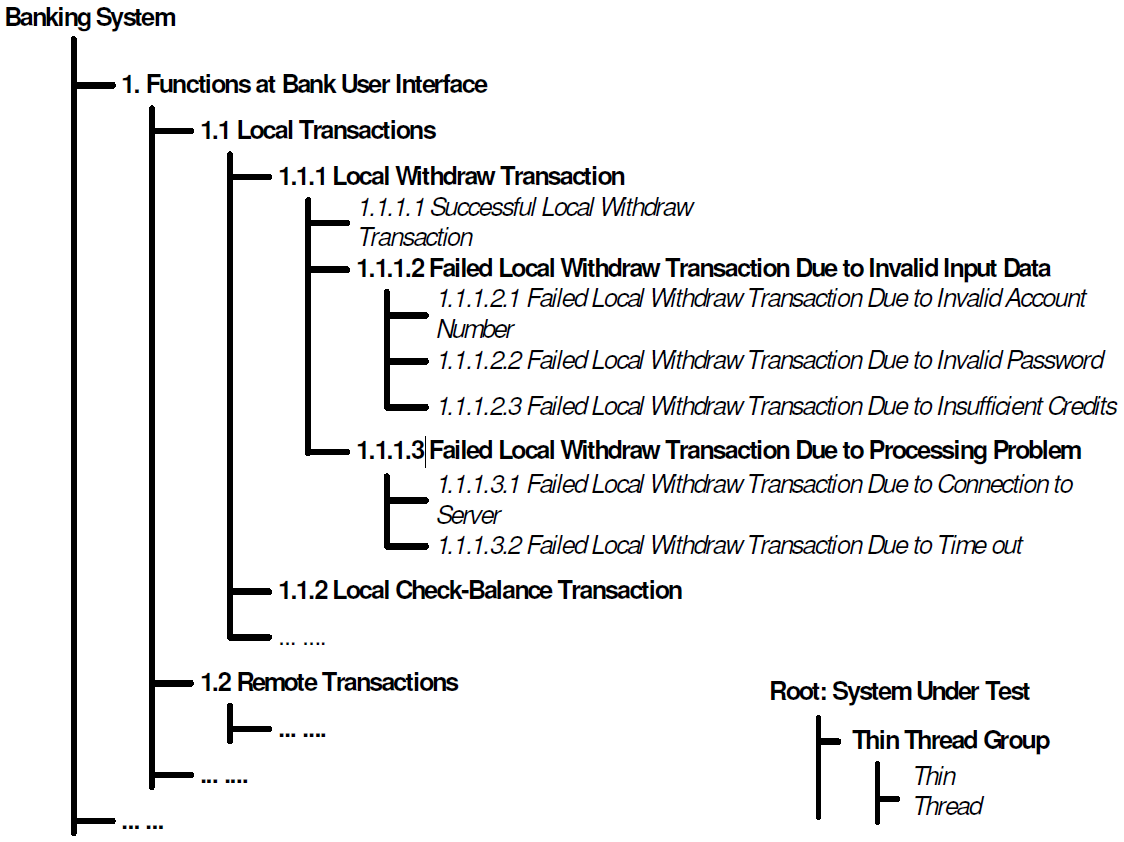
\includegraphics[scale=0.45]{img/Tsai2001ThinThreadTree.png}
    \caption{Een hypothetische thin-thread boom voor een bankiersapplicatie ~\cite{Tsai2001}}
    \label{fig:tsaithinthreadtree}
\end{figure}

De relaties tussen thin-threads onderling worden bepaald door hoe hun uitvoeringspaden zich tot elkaar verhouden:

\begin{enumerate}
    \item ``Deel-geheel'': het pad van één thin-thread is deel van dat van een andere thin-thread
    \item ``Identiek'': de paden zijn identiek; ze delen condities of andere eigenschappen
    \item ``Onafhankelijk'': de thin-threads hebben volledig andere paden
\end{enumerate}

Ook de condities kennen een reeks mogelijke verhoudingen:

\begin{enumerate}
    \item ``Onafhankelijk'': één conditie kan zich met of zonder een andere voordoen
    \item ``Gekoppeld'': één conditie kan of zal de andere veroorzaken
    \item ``Wederzijds uitgesloten'': slechts één van beide kan zich in één situatie voordoen
    \item ``Gerelateerd'': twee condities worden in dezelfde thin-thread gebruikt of sluiten elkaar uit
\end{enumerate}

Bij het opstellen van \textbf{E2E test cases} op basis van deze techniek dienen eerst de de thin-threads, hun condities, hun mogelijke input- en outputgegevens, en de relaties tussen de thin-threads en de condities onderling vastgelegd te worden. De test cases worden vervolgens opgebouwd uit individuele thin-threads. Thin-threads kunnen na elkaar uitgevoerd worden (``sequencing''), herhaald worden (``looping'') en op basis van voorwaarden uitgevoerd worden (``conditioned execution'').

\begin{figure}[h!]
    \centering
    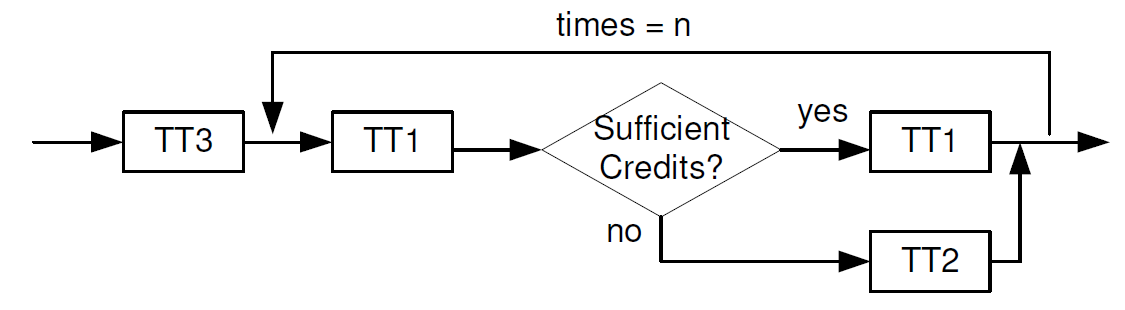
\includegraphics[scale=0.35]{img/Tsai2001ComplexTestScenario.png}
    \caption{Voorbeeld van een test case opgebouwd uit 3 verschillende thin-threads ~\cite{Tsai2001}}
    \label{fig:tsaicomplexscenario}
\end{figure}

Om de test cases te vervolledigen tot reële gebruiksscenario's moet men ten slotte inputs kiezen op basis van de grenzen van de condities. Meestal gaat men \emph{grenswaarden} kiezen om te testen \autocite{Jorgensen2013}, maar dit kan ook door: de input \emph{willekeurig} te selecteren \autocite{Loo1988}, de mogelijke inputs in \emph{categorieën} te sorteren en daar representatieve data uit halen of door eenvoudigweg data uit de reële gebruiksomgeving te gebruiken (\emph{``usage-based testing''}) \autocite{Dyer1992}.

\subsection{Overwegingen bij de Keuze voor een Test Automatisatiesysteem}

Test automatisatie vergt een substantiële initiële investering; analyse van de functionaliteit van de software, schrijven van testscripts, het introduceren van de tooling en het opleiden van personeel etc. \autocite{Kumar2016}. Het is dus van kritisch belang om een weloverwogen keuze te maken teneinde de kans op slagen van dergelijk project te maximaliseren. De volgende factoren zijn in het bijzonder belangrijk in acht te nemen:

\begin{itemize}
    \item \emph{De betrokken technologieën en omgevingen}. Het spreekt voor zich dat men voor het opzetten van test automatisatie anders te werk zal moeten gaan bij mainframe toepassingen dan voor webapplicaties. De beschikbare tooling zal ook afhankelijk zijn van de gebruikte technologieën (\cite{10.1145/1295014.1295062}).
    \item \emph{De beschikbare kennis}. Ervaring met een bepaald framework binnen het team is een sterke troef en vaak een doorslaggevende reden om een keuze te motiveren (\cite{Madan2013}).
    \item \emph{De lifecycle van de software}. Het te implementeren systeem dient te passen binnen het geplande levensverloop van de software zelf. Software waarvoor slechts een beperkt aantal toekomstige releases (of zelfs helemaal \emph{geen} toekomstige ontwikkeling) gepland is, zal niet gebaat zijn bij test automatisatie \autocite{Tiitinen2013}.
\end{itemize}

\section{e2e Testing Frameworks voor Angular}

\autocite{Anandan}
\autocite{Kumar2016}
\autocite{Barrett2013}
\autocite{Holmes}
\autocite{Singh2015}
\autocite{Madan2013}

\lipsum[4]

\subsection{Protractor}

\lipsum[6-7]

\subsection{Cypress}

\lipsum[3-4]

\subsection{UFT}

\lipsum[3-4]

\subsection{Behavior Driven Development Frameworks}

\lipsum[9]

\subsubsection{Mocha}

\lipsum[8-10]

\subsubsection{Jasmine \& Karma}

\lipsum[8-10]

\subsubsection{Cucumber}

\lipsum[8-10]
%%=============================================================================
%% Methodologie
%%=============================================================================

\chapter{\IfLanguageName{dutch}{Methodologie}{Methodology}}
\label{ch:methodologie}

%% TODO: Hoe ben je te werk gegaan? Verdeel je onderzoek in grote fasen, en
%% licht in elke fase toe welke stappen je gevolgd hebt. Verantwoord waarom je
%% op deze manier te werk gegaan bent. Je moet kunnen aantonen dat je de best
%% mogelijke manier toegepast hebt om een antwoord te vinden op de
%% onderzoeksvraag.

Het onderzoek steunt op twee benen: een literatuurstudie (hoofdstuk \ref{ch:stand-van-zaken}) enerzijds, en een reeks vergelijkende performantietesten van de drie kandidaat testautomatisatiesystemen (hoofdstuk \ref{ch:corpus}) anderzijds.

De literatuurstudie geeft — naast een bondig doch volledig overzicht van de grondlagen van test automatisatie — een resumé van de functionaliteiten en eigenschappen van de drie frameworks die door Colruyt Group overwogen worden. Dit onderdeel heeft niet alleen een belangrijk aandeel in het beantwoorden van de onderzoeksvraag; het is tevens het eerste deel van het voorbereidend werk dat aan het praktische luik van het onderzoek vooraf gaat.

%% ``resumé'' wordt hier gebruikt in de betekenis ``beknopt overzicht''

Het andere deel van het voorbereidend werk voor de performantietesten is de analyse van de werking van de UAT (application under test), die te vinden is in bijlage \ref{ch:functionele-omschrijving}. Aan de hand van deze functionele omschrijving is het mogelijk representatieve test cases te kiezen voor die testen.

Zoals ook blijkt uit de literatuurstudie vereist een test automatisatiesysteem een weloverwogen architectuur die dient als fundament voor het systeem. De opbouw van deze basis eist een aanzienlijke investering van tijd en voldoende bekendheid met het framework — de simulatie van randapparaten an sich is reeds een waardige kandidaat als onderwerp voor een verhandeling.

Om die reden wordt voor de performantietesten gebruik gemaakt van het bestaande werk van Thanuja Mudiyala (Test Automation Lead bij Colruyt Group Services) voor UFT en van Kenneth Aerens (Angular coach bij Colruyt Group Services) voor Cypress. De bestaande testen worden aangepast zodanig dat de stappen van elke test case precies dezelfde zijn. De implementatie van Protractor wordt volledig door de auteur gerealiseerd.

De 5 gekozen test cases die in elk framework worden uitgevoerd, zijn als volgt:

\begin{enumerate}
    \item \emph{Operator aanloggen}
    \item \emph{Artikel toevoegen}
    \item \emph{Handscanner gebruiken}
    \item \emph{Factuur maken}
    \item \emph{Betaling registreren}
\end{enumerate}

%% Gewichtsregistraties werden uitgesloten van de testen omdat de certifiëring van de weegschaal nog niet op punt stond.

Elk framework wordt geconfigureerd zodanig dat deze 5 testen na elkaar worden uitgevoerd, zoals ook het geval zou zijn bij het normale gebruik van het test automatisatiesysteem. Het voorbereidende werk hiervoor, alsook de relevante details van de uitvoering, worden in hoofdstuk \ref{ch:corpus} besproken. Ook worden eigenschappen en mogelijkheden van de frameworks getoetst aan de requirement die door Colruyt Group vooropgesteld worden, zie sectie \ref{sec:meth-requirements}.

Tijdens de performantietesten wordt gebruik gemaakt van Windows \textsuperscript{\textregistered} Performance Monitor (ook gekend als ``PerfMon'') om de performantie van de frameworks te meten. Om dit te bereiken worden de processen die relevant zijn voor het uitvoeren van de testen in elk framework geïdentificeerd. Van deze processen wordt tijdens de uitvoer van de testen volgende metrieken gelogd:

\begin{enumerate}
    \item \emph{Elapsed Time}: de verlopen tijd sinds het starten van het proces, in seconden.
    \item \emph{\% Processor Time}: het aandeel van de verlopen tijd die de processor aan de processen besteed (\cite{Tarra2014}).
    \item \emph{Private Bytes}: de totale hoeveelheid geheugen dat aan de processen gealloceerd wordt, in bytes (\cite{Hudek2017}).
    \item \emph{Virtual Bytes}: de totale hoeveelheid geheugen die effectief door de processen benut wordt, in bytes (\cite{Hudek2017}).
    \item \emph{Thread Count}: het aantal processor threads die door de processen gebruikt worden (\cite{Satran2018}).
    \item \emph{Handle Count}: het aantal toegangen tot systeembronnen die de processen vasthouden.
\end{enumerate}

%% Gebruik van PerfMon:
%% 1. Run... perfmon.exe
%% 2. Ga naar Monitoring Tools > Performance Monitor en voeg counters toe, alsook instances van processen
%% 3. Rechtsklik op Performance Monitor New > Data Collector Set
%% 4. Rechtsklik op Data Collector Sets > User Defined > [YourDataCollectorSet] en klik Start om opname te starten
%% 5. Idem, maar Stop om te stoppen
%% 6. Open cmd.exe
%% 7. Gebruik cd om naar de directory van [YourDataCollectorSet] te gaan
%% 8. Zet .blg naar .csv om met commando 'relog MyMonitorLog.blg -f csv -o MyMonitorLog.csv'

De gedetailleerde resultaten van deze testen zijn te vinden in bijlage \ref{ch:resultaten} en worden vervolgens onderworpen aan statistische analyse in sectie \ref{sec:analyse-performantietesten}. In sectie \ref{sec:resultaten-requirements} wordt vervolgens besproken in welke mate de frameworks onderling aan de in sectie \ref{sec:meth-requirements} vooropgestelde requirements voldoen.

Het onderzoek wordt ten slotte afgesloten met de conclusie. Dit hoofdstuk bevat het advies dat aan Colruyt Group voorgelegd wordt als antwoord op de onderzoeksvraag.

\section{Requirementsanalyse}
\label{sec:meth-requirements}

De requirementsanalyse is een vast onderdeel voor een vergelijkende studie. De voor dit onderzoek geldende requirements werden vastgelegd op 5 maart 2020 met input van Koen Stockman (applicatiemanager en co-promotor van deze verhandeling) en Kenneth Aerens (Angular coach voor Colruyt Group) en kan men hieronder vinden. De requirements werden opgesplitst in functionele\footnote{Functionele requirements zijn de eisen die gesteld worden aan de beschikbare functionaliteiten en objectieve eigenschappen van een systeem} en niet-functionele\footnote{Niet-functionele requirements zijn kwaliteitseisen die gekoppeld worden aan een zinvolle metriek.} vereisten.

\textbf{Functionele requirements}:
\begin{itemize}
    \item \emph{Moet} compatibel zijn met Angular en Angular applicaties
    \item \emph{Moet} compatibel zijn met de Chrome browser
    \item \emph{Moet} de mogelijkheid bieden randapparaten te simuleren
    \item \emph{Moet} auto-synchronisatie (automatisch wachten) aanbieden
    \item \emph{Moet} hergebruik van componenten en handelingen mogelijk maken
    \item Vereist \emph{idealiter} geen (of toch zo weinig mogelijk) externe technologieën zoals een losstaande web driver.
    \item Is \emph{idealiter} integreerbaar in Visual Studio Code, de IDE\footnote{Integrated Development Environment} die Colruyt Group gebruikt voor Angular ontwikkeling.
    \item Ondersteunt \emph{idealiter} meerdere assertion libraries.
    \item Gebruikt \emph{idealiter} een op Java of JavaScript gebaseerde taal voor de programmatie.
\end{itemize}

\textbf{Niet-functionele requirements}:
\begin{itemize}
    \item \emph{Moet} (relatief) goedkoop zijn in zowel opzet als onderhoud
    \item \emph{Moet} voldoende performant zijn om een groot aantal testen snel te kunnen verwerken
    \item \emph{Moet} een (relatief) vlakke leercurve hebben.
    \item Blijft in de toekomst \emph{idealiter} ondersteund door de ontwikkelaar\footnote{Colruyt Group maakte tot voor kort uitgebreid gebruik van de programmeertaal ObjectStar, die intussen niet meer ondersteund was. Het herschrijven van alle applicaties en systeem die gebruikt maakten van ObjectStar was een enorme kost die Colruyt niet opnieuw wil maken.}
\end{itemize}
%%=============================================================================
%% Corpus
%%=============================================================================

\chapter{\IfLanguageName{dutch}{Corpus}{Corpus}}
\label{ch:corpus}

\section{Protractor}

\subsection{Structuur Project}

\subsection{Uitvoering Praktijktest}

\subsection{Requirements}

\section{Cypress}

\subsection{Structuur Project}

\subsection{Uitvoering Praktijktest}

\subsection{Requirements}

\section{UFT}

\subsection{Structuur Project}

\subsection{Uitvoering Praktijktest}

\subsection{Requirements}
%%=============================================================================
%% Verwerking resultaten
%%=============================================================================

\chapter{Verwerking Resultaten}
\label{ch:verwerking-resultaten}

\section{Analyse Resultaten Performantietesten}
\label{sec:analyse-performantietesten}

\section{Resultaten Requirements}
\label{sec:resultaten-requirements}

% Voeg hier je eigen hoofdstukken toe die de ``corpus'' van je bachelorproef
% vormen. De structuur en titels hangen af van je eigen onderzoek. Je kan bv.
% elke fase in je onderzoek in een apart hoofdstuk bespreken.

%\input{...}
%\input{...}
%...

%%=============================================================================
%% Conclusie
%%=============================================================================

\chapter{Conclusie}
\label{ch:conclusie}

% TODO: Trek een duidelijke conclusie, in de vorm van een antwoord op de
% onderzoeksvra(a)g(en). Wat was jouw bijdrage aan het onderzoeksdomein en
% hoe biedt dit meerwaarde aan het vakgebied/doelgroep? 
% Reflecteer kritisch over het resultaat. In Engelse teksten wordt deze sectie
% ``Discussion'' genoemd. Had je deze uitkomst verwacht? Zijn er zaken die nog
% niet duidelijk zijn?
% Heeft het onderzoek geleid tot nieuwe vragen die uitnodigen tot verder 
%onderzoek?

Colruyt Group heeft de keuze tussen 3 heel geschikte frameworks — er is geen verkeerde keuze. Dat gezegd zijnde wordt Colruyt Group aangeraden om te kiezen voor \textbf{Cypress}, met \textbf{Protractor} als tweede keuze.

UFT is weliswaar een robuust framework, maar het heeft een aantaal belangrijke nadelen:

\begin{itemize}
    \item De hoge licentiekost, die voor een kostenbewuste firma als Colruyt Group niet aantrekkelijk is.
    \item De steile leercurve. Geen van de programmeurs die de end-to-end testen voor TAC2.0 zullen schrijven, hebben ervaring met UFT. Hen leren werken met het pakket zou dus een bijkomende investering zijn.
    \item UFT is beduidend trager in uitvoer — wat geen ideale situatie is gezien Colruyt Group met zijn IT landschap richting containerization en continuous deployment wil gaan.
\end{itemize}

De keuze tussen Protractor of Cypress is iets minder evident. Protractor heeft als voordelen dat het meer zekerheid biedt naar de toekomst toe (het wordt ontwikkeld door Google) en dat het iets matuurder is dan Cypress. Cypress, daarentegen, vereist geen ondersteunende software. Bovendien geniet Cypress de voorkeur van het team, onder leiding van Angular coach Kenneth Aerens. De literatuur wees al aan dat de aanvaarding van het gekozen framework van kritisch belang is voor het succes van een project.

Dit geheel aan feiten motiveert het advies om te kiezen voor Cypress als end-to-end testing framework, met Protractor als tweede keuze.

Dit resultaat is niet geheel onverwacht — de nadelen van UFT zijn goed gekend en waren ook de motivatie voor Colruyt Group om andere kandidaten te overwegen.

Toch zijn er nog een aantal openstaande vragen. Eerst en vooral vonden er voor Protractor geen praktijktesten plaats, wat maakt dat dit advies niet met 100\% zekerheid gegeven kan worden. Ten tweede is het niet duidelijk wat de impact was van de verschillende methodes om de randapparaten te simuleren — deze variabelen was idealiter niet aanwezig in de performantietesten. Ten slotte werden de testen uitgevoerd met een live pre-productie backend; het is niet duidelijk of dit een invloed had op de testen, hoewel het de implementatie alleszins bemoeilijkt heeft.

Zij die dit onderzoek willen gebruiken als basis voor hun eigen vergelijkende studie wordt afgeraden om te werken met de productiesoftware. De complexiteiten die daarmee gepaard gaan — in dit geval interfacing met randapparaten, een gedeelde databank, afhankelijkheden met andere systemen, eventuele moeilijkheden met licenties en security etc. — leiden af van de kern van het onderzoek. In de plaats daarvan wordt het aangeraden een minimaal prototype van de applicatie te werken zodat deze externe factoren uitgeschakeld kunnen worden.


%%=============================================================================
%% Bijlagen
%%=============================================================================

\appendix
\renewcommand{\chaptername}{Appendix}

%%---------- Onderzoeksvoorstel -----------------------------------------------

\chapter{Onderzoeksvoorstel}

Het onderwerp van deze bachelorproef is gebaseerd op een onderzoeksvoorstel dat vooraf werd beoordeeld door de promotor. Dat voorstel is opgenomen in deze bijlage.

% Verwijzing naar het bestand met de inhoud van het onderzoeksvoorstel
%---------- Inleiding ---------------------------------------------------------

\section{Introductie} % The \section*{} command stops section numbering
\label{sec:introductie}
Het correct én efficiënt verwerken van klantenaankopen is een cruciaal process binnen de retailsector. Om die reden investeert Colruyt Group momenteel in nieuwe touchscreens voor haar voornaamste kassasysteem, alsook een herwerking van de checkoutsoftware.

Hoewel de ontwikkeling van deze software met rasse schreden vooruit gaat, werd er tot op heden maar weinig geïnvesteerd in (geautomatiseerde) e2e (end to end, oftewel een simulatie van een echt gebruikersscenario waarbij alle componenten van het systeem getest worden ~\cite{SoftwareTestingHelp2019}) testing. Nochtans is de stabiliteit van het kassasysteem een onbetwistbare noodzaak voor groep.

Bovendien wordt de software continu uitgebreid met nieuwe functionaliteit en moet het probleemloos kunnen interfacen met een waslijst aan andere systemen (barcodelezers, weegschalen, betaalterminals, de systemen van stockbeheer, productinformatie, finance, customer relations, marketing \& promotie etc.).
\vspace{\baselineskip}
Een robuust testsysteem is bijgevolg onontbeerlijk en ondersteunt de softwareontwikkeling door:

\begin{itemize}
  \item het vroegtijdig onderscheppen van defecten
  \item een grotere test coverage
  \item een grotere efficiëntie van testen
  \item een snellere time-to-market
  \item een verlaging van de ontwikkelingskosten
\end{itemize}

De eerste stap voor het uitbouwen van een testsysteem is het kiezen van een gepast testing framework. Ook voor een relatief jong framework zoals Angular zijn er reeds verschillende alternatieven beschikbaar.
\vspace{\baselineskip}
Het onderzoek dat onderwerp is van dit voorstel bestaat er dus uit om na te gaan:

\begin{itemize}
    \item welke e2e (end to end, d.w.z. testen die gebruik in een productie-omgeving simuleren) testing frameworks bestaan voor Angular en welke randvoorwaarden (kost, beschikbare ondersteuning en documentatie, vereiste programmeervaardigheden) zij hebben,
    \item in welke mate de bestaande frameworks de volledige functionaliteit van het systeem kunnen afdekken,
    \item hoe performant elk van de frameworks is en
    \item hoe betrouwbaar de resultaten van de frameworks zijn
\end{itemize}

om zo het meest geschikte framework voor de use case van Colruyt Group te kunnen aanbevelen.

%---------- Stand van zaken ---------------------------------------------------

\section{State-of-the-art}
\label{sec:state-of-the-art}

De keuze voor een geschikt e2e testing framework is sterk afhankelijk van de specifieke context waarbinnen dit gebruikt gaat worden. Colruyt Group overweegt momenteel 2 verschillende frameworks:

\begin{itemize}
    \item \textbf{Protractor} — een API voor e2e testing die steunt op Selenium (een ``WebDriver'' die webapplicaties voor testdoeleinden automatiseert)
    \item \textbf{Cypress} — een relatief nieuw e2e framework
\end{itemize}

\vspace{\baselineskip}

Daarnaast zijn er nog een reeks andere Behavior-Driven Development of testing frameworks voor het JavaScript ecosysteem. De meest prominente frameworks die van toepassing zijn op Angular, buiten bovenstaande, zijn de volgende:

\begin{itemize}
    \item \textbf{Jasmine}
    \item \textbf{Jest}
    \item \textbf{Mocha}
    \item \textbf{Puppeteer}
    \item \textbf{AVA}
    \item \textbf{Cucumber}
\end{itemize}

\vspace{\baselineskip}

Zie ook ~\cite{Castro2019}; ~\cite{Definition2019}; ~\cite{Kamalizade2019}; ~\cite{Lotanna2019}; ~\cite{Roy2019} en ~\cite{Zaidman2019}.

%Hier beschrijf je de \emph{state-of-the-art} rondom je gekozen onderzoeksdomein. Dit kan bijvoorbeeld een literatuurstudie zijn. Je mag de titel van deze sectie ook aanpassen (literatuurstudie, stand van zaken, enz.). Zijn er al gelijkaardige onderzoeken gevoerd? Wat concluderen ze? Wat is het verschil met jouw onderzoek? Wat is de relevantie met jouw onderzoek?

%Verwijs bij elke introductie van een term of bewering over het domein naar de vakliteratuur, bijvoorbeeld~\autocite{Doll1954}! Denk zeker goed na welke werken je refereert en waarom.

% Voor literatuurverwijzingen zijn er twee belangrijke commando's:
% \autocite{KEY} => (Auteur, jaartal) Gebruik dit als de naam van de auteur
%   geen onderdeel is van de zin.
% \textcite{KEY} => Auteur (jaartal)  Gebruik dit als de auteursnaam wel een
%   functie heeft in de zin (bv. ``Uit onderzoek door Doll & Hill (1954) bleek
%   ...'')

%Je mag gerust gebruik maken van subsecties in dit onderdeel.

%---------- Methodologie ------------------------------------------------------
\section{Methodologie}
\label{sec:methodologie}

Om het meest geschikte framework voor Colruyt Group's checkoutsysteem te kunnen identificeren, dienen volgende stappen genomen te worden:

\begin{enumerate}
    \item onderzoek naar de \textbf{mogelijkheden en randvoorwaarden} van elke kandidaat, om daar de 3 meest geschikte kandidaten uit te halen
    \item onderzoek naar de \textbf{huidige functionaliteit} van het kassasysteem, alsook de bestaande interfacing met randapparaten en andere systemen
    \item de selectie van een \textbf{representatieve subset} van de functionaliteit van het kassasysteem
    \item schrijven van \textbf{identieke testscenario's} in elk van de 3 gekozen testing frameworks
    \item opzetten van de frameworks, \textbf{uitvoeren van de testscenario's} en meten van de performantie (complexiteit van installatie, benodigde tijd om testen te schrijven, doorlooptijd, geheugengebruik)
    \item formuleren van een \textbf{advies} op basis van de gegevens verzameld in de voorgaande stappen
\end{enumerate}
\vspace{\baselineskip}
Dit advies is het eindresultaat van dit onderzoek.

%Hier beschrijf je hoe je van plan bent het onderzoek te voeren. Welke onderzoekstechniek ga je toepassen om elk van je onderzoeksvragen te beantwoorden? Gebruik je hiervoor experimenten, vragenlijsten, simulaties? Je beschrijft ook al welke tools je denkt hiervoor te gebruiken of te ontwikkelen.

%---------- Verwachte resultaten ----------------------------------------------
\section{Verwachte resultaten}
\label{sec:verwachte_resultaten}

De resultaten voor dit onderzoek zijn moeilijk te anticiperen omwille van het veelvoud aan variabelen die van toepassing zijn. Elk van de verschillende testingframeworks zal vermoedelijk voor- en nadelen hebben en het uiteindelijke advies zal afhangen van de specifieke behoeften van Colruyt Group en de eigenschappen van het Checkoutsysteem.

Naast een overzicht van de mogelijkheden en randvoorwaarden van elk testing framework, zullen de resultaten van de testscenario's een objectief beeld van de voor- en nadelen van elk framework kunnen geven.

    \begin{figure}[h!]
    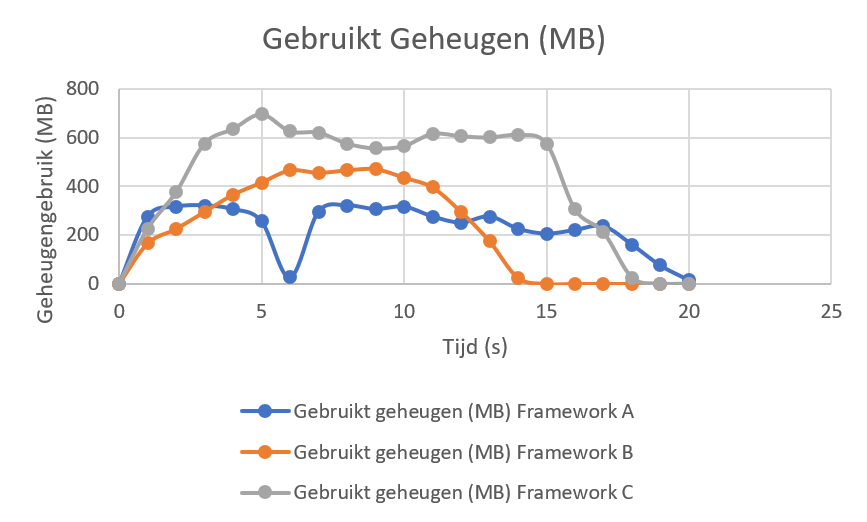
\includegraphics[width=\linewidth]{img/gebruiktgeheugen.PNG}
    \caption{Mock grafiek: Geheugengebruik in MB van de verschillende testframeworks tijdens het uitvoeren van de testscenario's.}
    \label{fig:geheugenmock}
    \end{figure}

    \begin{figure}[h!]
    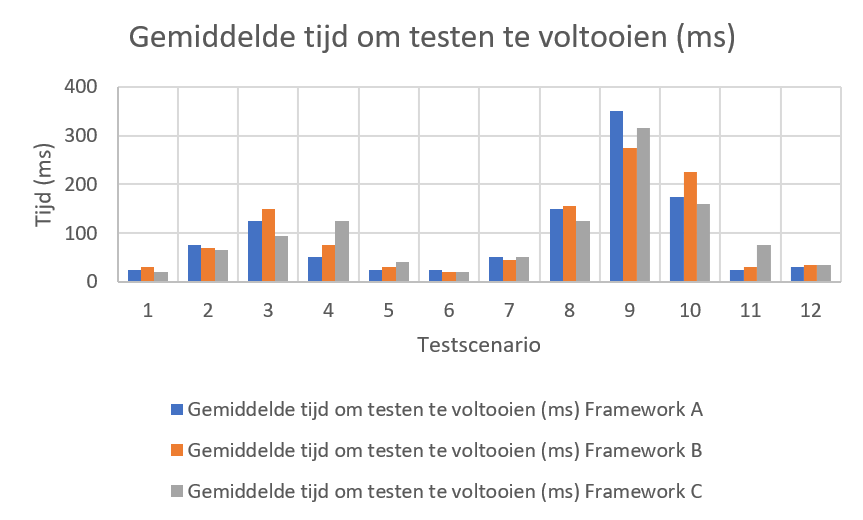
\includegraphics[width=\linewidth]{img/gemtijdtestenvoltooien.PNG}
    \caption{Mock grafiek: Benodigde tijd om elk van de verschillende testscenario's uit te voeren.}
    \label{fig:uitvoertijdmock}
    \end{figure}

%Hier beschrijf je welke resultaten je verwacht. Als je metingen en simulaties uitvoert, kan je hier al mock-ups maken van de grafieken samen met de verwachte conclusies. Benoem zeker al je assen en de stukken van de grafiek die je gaat gebruiken. Dit zorgt ervoor dat je concreet weet hoe je je data gaat moeten structureren.

%---------- Verwachte conclusies ----------------------------------------------
\section{Verwachte conclusies}
\label{sec:verwachte_conclusies}

Zoals reeds eerder vermeldt, is het moeilijk om in te schatten welk framework uiteindelijk geadviseerd zal worden. De ontwikkelaars van het Checkoutsysteem lijkt in eerste instantie de voorkeur te geven aan het recentere Cypress, vooral omdat testen schrijven in dit framework intuïtiever en sneller zou zijn. In welke mate een framework aanvaard wordt is vaak de doorslaggevende factor om een bepaald framework te kiezen, en het lijkt dus aannemelijk dat Cypress uiteindelijk opgenomen wordt in het advies.

%Hier beschrijf je wat je verwacht uit je onderzoek, met de motivatie waarom. Het is \textbf{niet} erg indien uit je onderzoek andere resultaten en conclusies vloeien dan dat je hier beschrijft: het is dan juist interessant om te onderzoeken waarom jouw hypothesen niet overeenkomen met de resultaten.



%%---------- Andere bijlagen --------------------------------------------------
% TODO: Voeg hier eventuele andere bijlagen toe
%%=============================================================================
%% Inleiding
%%=============================================================================

\chapter{\IfLanguageName{dutch}{Functionele Omschrijving TAC2.0}{Functional Description TAC2.0}}
\label{ch:functionele-omschrijving}

Het checkoutsysteem van Colruyt Group is een complex gegeven dat bestaat uit een verscheidenheid aan individuele componenten en verwoven zit met zo goed als elk facet van de firma. Een grondige kennis van dit systeem, en in het bijzonder de werking van het systeem vanuit het perspectief van de kassabediende, is dan ook onontbeerlijk voor dit onderzoek.

\section{Algemeen}

In de filialen van Colruyt, Colruyt France, OKay, OKay City, Bio-Planet, Dreamland, Dreambaby, en Colruyt Group Spar worden klantenaankopen verwerkt middels de \textbf{TAC} (``tactile'') schermen.

[randapparaten]

[]

[filiaalserver draait applicaties buiten FVS, DB wordt gebruikt voor data die niet-FVS is... FVS is meer dan enkel de TAC]

\section{Kassaproces}

Colruyt Group is een sterk procesgerichte organisatie; 

Registreren en afhandelen van klantenaankoop < Verkopen van goederen < Verkoop

\section{Lorem Ipsum}

#
%%=============================================================================
%% Cypress Code
%%=============================================================================

\chapter{\IfLanguageName{dutch}{Cypress Test Cases}{Cypress Test Cases}}
\label{ch:code-cypress}

\section{Operator Aanloggen}

\begin{minted}[
linenos,
breaklines
]
{JavaScript}
Feature: Authenticate

@focus
Scenario Outline: : Authenticate CTAC operator
Given Open xtac as <tacType> <tacId> <tacSubType>
When I click on button Ctac
And I authenticate as operator <operator> and password <password>
Then Url should be "xtac/ctac/transaction"
Examples:
| tacType | tacId | tacSubType | operator | password |
| CTAC    | 1     |            | 10       | false    |
| KTAC    | 1     |            | 11       | false    |
| MTAC    | 1     |            | 12       | false    |

#      | MTAC    | 3     | A          | 13       | false     |
#      | MTAC    | 4     | B          | 14       | false    |

#      | MTAC    | 4     | aspar      | 31       | false    |
#      | ATAC    | 2     | codifr     | 99       | false    |
#      | CTAC    | 2     | codifr     | 99       | false    |
#      | KTAC    | 2     | codifr     | 99       | false    |
#      | MTAC    | 2     | codifr     | 99       | false    |


#  @focus
Scenario Outline: : Authenticate PTAC operator
Given Open xtac as <tacType> <tacId> <tacSubType>
When I click on button Ptac
And I authenticate as operator <operator> and password <password>
Then Url should be "xtac/ptac/payment"

Examples:
| tacType | tacId | tacSubType | operator | password |
| PTAC    | 1     |            | 20       | false    |
| KTAC    | 1     |            | 21       | false    |
| MTAC    | 1     |            | 99       | false    |
#      | MTAC    | 3     | dreamland  | 99       | 11       |
#      | MTAC    | 4     | spar       | 99       | false    |
#      | MTAC    | 4     | aspar      | 99       | false    |
#      | ATAC    | 2     | codifr     | 99       | false    |
#      | PTAC    | 2     | codifr     | 99       | false    |
#      | KTAC    | 2     | codifr     | 99       | false    |
#      | MTAC    | 2     | codifr     | 99       | false    |
\end{minted}

\section{Artikel Toevoegen}

\begin{minted}[
linenos,
breaklines
]
{JavaScript}






Feature: Add article to transaction

@focus
Scenario Outline: I follow the happy add article flow
Given Open xtac as <tacType> <tacId> <tacSubType>
When I authenticate as operator <operatorId> and password <password> on "Ctac"
Then Url should be "xtac/ctac/transaction"
And TransactionList should have <totalColumns> columns
And TransactionList should have 5 rows
And Buttons <additionButtons> should be disabled
And Button <subBill> should be disabled
When I click on button "BUTTON.ARTICLE_NR"
Then Url should be "xtac/ctac/transaction/article-details"
And Button-list ".button-salesActionButtons" should be disabled
When I add article 5006
Then Input <field> should have value <field_value>
And Button <subBill> should be enabled
When I click on button "BUTTON.ARTICLE_NR"
Then Buttons <additionButtons> should be disabled
And Button "BUTTON.PAY" should be disabled
And Input article_nr should have value ""
And TransactionList row 4 column 2 should look like <column3>
And TransactionList row 4 column 1 should look like <column2>
When I add article 5006
Then Input <field> should have value <field_value>
And Button <subBill> should be enabled
When I click on button "BUTTON.ARTICLE_NR"
Then Input article_nr should have value ""
And Buttons <additionButtons> should be disabled
And TransactionList row 3 column 2 should look like <column3>
And TransactionList row 3 column 1 should look like <column2>
And TransactionList row 4 column 2 should look like <column3>
And TransactionList row 4 column 1 should look like <column2>


Examples:
| tacType | tacId | tacSubType | operatorId | password | field            | field_value | totalColumns | column2                    | column3 | subBill           | additionButtons                                 |
| CTAC    |  1    |            | 99         | false    | article_quantity | "1"         | 3            | "€ 6,89  \\\| tot: € 6,89" | "1 * 1" | "BUTTON.SUB_BILL" | "BUTTON.SPECIAL_PRICE, BUTTON.PERCENT_DISCOUNT" |
| MTAC    |  1    |            | 98         | false    | article_quantity | "1"         | 3            | "€ 6,89  \\\| tot: € 6,89" | "1 * 1" | "BUTTON.SUB_BILL" | "BUTTON.SPECIAL_PRICE, BUTTON.PERCENT_DISCOUNT" |
| KTAC    |  1    |            | 81         | false    | article_quantity | "1"         | 3            | "€ 6,89  \\\| tot: € 6,89" | "1 * 1" | "BUTTON.SUB_BILL" | "BUTTON.SPECIAL_PRICE, BUTTON.PERCENT_DISCOUNT" |
#      | MTAC    |  3    | dreamland  | 99         | 11       | article_quantity   | "1"         | 3            | "€ 6,89"                   | "1"     | "BUTTON.SUB_BILL" | "BUTTON.PERCENT_DISCOUNT"                       |
#      | MTAC    |  3    | dreamland  | 99         | 11       | article_unit_price | "6,89"      | 3            | "€ 6,89"                   | "1"     | "BUTTON.SUB_BILL" | "BUTTON.PERCENT_DISCOUNT"                       |
#      | MTAC    |  4    | spar       | 99         | false    | article_quantity   | "1"         | 3            | "€ 6,89  \\\| tot: € 6,89" | "1 * 1" | "BUTTON.PARKING"  | "BUTTON.PERCENT_DISCOUNT"                       |
#      | KTAC    |  2    | codifr     | 99         | false    | article_quantity   | "1"         | 3            | "€ 6,89  \\\| tot: € 6,89" | "1 * 1" | "BUTTON.SUB_BILL" | "BUTTON.PERCENT_DISCOUNT"                       |
#      | CTAC    |  2    | codifr     | 99         | false    | article_quantity   | "1"         | 3            | "€ 6,89  \\\| tot: € 6,89" | "1 * 1" | "BUTTON.SUB_BILL" | "BUTTON.PERCENT_DISCOUNT"                       |
\end{minted}

\section{Handscanner Gebruiken}

\begin{minted}[
linenos,
breaklines
]
{JavaScript}
Feature: Scan an article

@focus
Scenario Outline: I scan an article with the hand scanner
Given Open xtac as <tacType> <tacId> <tacSubType>
When I authenticate as operator <operatorId> and password <password> on "Ctac"
Then Url should be "xtac/ctac/transaction"
When I scan article 5412476144501
And I scan article 5412476042654
Then Url should be "xtac/ctac/transaction/article-details"
And Input <field> should have value <field_value>
And TransactionList row 4 column 2 should look like <column3>
And TransactionList row 4 column 1 should look like <column2>
When I click on button BUTTON.ARTICLE_NR
Then TransactionList row 3 column 2 should look like <column3>
And TransactionList row 3 column 1 should look like <column2>
And TransactionList row 4 column 2 should look like "1 * 1"
And TransactionList row 4 column 1 should look like "€ 7,41 | tot: € 7,41"


Examples:
| tacType | tacId | tacSubType | operatorId | password | field            | field_value | column2                    | column3 | subBill           | additionButtons                                 |
| CTAC    |  1    |            | 5          | false    | article_quantity | "1"         | "€ 1,96  \\\| tot: € 1,96" | "1 * 1" | "BUTTON.SUB_BILL" | "BUTTON.SPECIAL_PRICE, BUTTON.PERCENT_DISCOUNT" |
#      | MTAC    |  1    |            | 6          | false    | article_quantity | "1"         | "€ 1,96  \\\| tot: € 1,96" | "1 * 1" | "BUTTON.SUB_BILL" | "BUTTON.SPECIAL_PRICE, BUTTON.PERCENT_DISCOUNT" |
#      | KTAC    |  1    |            | 7          | false    | article_quantity | "1"         | "€ 1,96  \\\| tot: € 1,96" | "1 * 1" | "BUTTON.SUB_BILL" | "BUTTON.SPECIAL_PRICE, BUTTON.PERCENT_DISCOUNT" |
#      | MTAC    |  3    | dreamland  | 99         | 11       | article_quantity   | "1"         | "€ 6,89"                   | "1"     | "BUTTON.SUB_BILL" | "BUTTON.PERCENT_DISCOUNT"                       |
#      | MTAC    |  3    | dreamland  | 99         | 11       | article_unit_price | "6,89"      | "€ 6,89"                   | "1"     | "BUTTON.SUB_BILL" | "BUTTON.PERCENT_DISCOUNT"                       |
#      | MTAC    |  4    | spar       | 99         | false    | article_quantity   | "1"         | "€ 6,89  \\\| tot: € 6,89" | "1 * 1" | "BUTTON.PARKING"  | "BUTTON.PERCENT_DISCOUNT"                       |
#      | KTAC    |  2    | codifr     | 99         | false    | article_quantity   | "1"         | "€ 6,89  \\\| tot: € 6,89" | "1 * 1" | "BUTTON.SUB_BILL" | "BUTTON.PERCENT_DISCOUNT"                       |
#      | CTAC    |  2    | codifr     | 99         | false    | article_quantity   | "1"         | "€ 6,89  \\\| tot: € 6,89" | "1 * 1" | "BUTTON.SUB_BILL" | "BUTTON.PERCENT_DISCOUNT"                       |


#  @focus
Scenario Outline: I scan a supplier coupon with the hand scanner
Given Open xtac as <tacType> <tacId> <tacSubType> and continue
When I authenticate as operator <operatorId> and password <password> on "Ctac"
Then Url should be "xtac/ctac/transaction"
When I scan article <article1>
Then Url should be "xtac/ctac/transaction/article-details"
When I scan article <article2>
Then Url should be "xtac/ctac/transaction/article-details"
And I <get_warning> get a warning <warn_msg>
When I <get_warning> choose option number 1
Then Input <field> should have value <field_value>
And TransactionList row 4 column 2 should look like <column3>
And TransactionList row 4 column 1 should look like <column2>
When I click on button BUTTON.ARTICLE_NR
Then TransactionList row 3 column 2 should look like <column3>
And TransactionList row 3 column 1 should look like <column2>
And TransactionList row 4 column 0 should look like <column1>
And TransactionList row 4 column 0 should look like <column1-info>

Examples:
| tacType | tacId | tacSubType | operatorId | password | article1      | article2                      | get_warning | warn_msg                                       | field         | field_value                              | column1           | column1-info      | column2                    | column3 |
#      | CTAC    |  1    |            | 5          | false    | 5412476144501 | 9826042110009 |             | "GRATIS leveranciersbon" | article_name  | "Leveranciersbon"                        | "Leveranciersbon" | "1 stuk gratis"   | "€ 1,96  \\\| tot: € 1,96" | "1 * 1" |
#      | CTAC    |  1    |            | 5          | false    | 5412476144501 | 9820094740306 | don't       |                          | article_name  | "Leveranciersbon       Bedrag: € -0,30"  | "Leveranciersbon" | "Bedrag: € -0,30" | "€ 1,96  \\\| tot: € 1,96" | "1 * 1" |
#      | CTAC    |  1    |            | 5          | false    | 5412476144501 | 9820094740757 | don't       |                          | article_name  | "Leveranciersbon       Bedrag: € -0,75"  | "Leveranciersbon" | "Bedrag: € -0,75" | "€ 1,96  \\\| tot: € 1,96" | "1 * 1" |
#      | CTAC    |  1    |            | 5          | false    | 5412476144501 | 9820094743758 |             | "Bedrag leveranciersbon" | article_name  | "Leveranciersbon       Bedrag: € -3,75"  | "Leveranciersbon" | "Bedrag: € -3,75" | "€ 1,96  \\\| tot: € 1,96" | "1 * 1" |
| CTAC    |  1    |            | 5          | false    | 5413149191228 | ]C12555400100000002\"39021000 |             | "Bedrag leveranciersbon  \\\| Bedrag: € -10,00" | article_name  | "Leveranciersbon       Bedrag: € -3,75"  | "Leveranciersbon" | "Bedrag: € -3,75" | "€ 1,96  \\\| tot: € 1,96" | "1 * 1" |

#  @focus
Scenario: I scan a supplier coupon that needs manual reduction input
Given Open xtac as CTAC 1  and continue
When I authenticate as operator 14 and password false on "Ctac"
Then Url should be "xtac/ctac/transaction"
When I scan article 5412476144501
Then Url should be "xtac/ctac/transaction/article-details"
When I scan article 9820094743758
Then Url should be "xtac/ctac/transaction/article-details"
And I  get a warning "Bedrag leveranciersbon"
When I  choose option number 2
Then Input article_name should have value "Leveranciersbon"
And Input article_reduction_price should have value ""
When I enter reduction 2,00
Then Input article_reduction_price should have value "2,00"
When I click on button BUTTON.ARTICLE_NR
Then TransactionList row 4 column 0 should look like "Leveranciersbon"
And TransactionList row 4 column 0 should look like "Bedrag: € -2,00"
And TransactionList row 4 column 2 should look like "1 * 1"
\end{minted}

\section{Factuur Maken}

\begin{minted}[
linenos,
breaklines
]
{JavaScript}
import { authenticate } from '../../support/authenticate/user';
import { input } from '../../support/input';
import { MODAL } from '../../support/modal/button';
import { clickButton } from '../../support/step_definitions/click-on-button';
import { INVOICE } from './invoice';

describe('Discount article', () => {
    beforeEach(() => {
        cy.visit('?tacType=ctac&tacId=1');
        authenticate('1', undefined, 'ctac1');
        clickButton(INVOICE.button);
        });

    it('should select the first control again', () => {
        clickButton(INVOICE.search.streetPostal);

        input(INVOICE.input.street).hasFocus()
            .enterValue('KERKSTRAAT').hasValue('KERKSTRAAT')
            .submit();

        input(INVOICE.input.postalCode).hasError()
            .enterValue('8500').hasValue('8500').submit();

        clickButton(MODAL.button.back);

        input(INVOICE.input.street).hasFocus();

        clickButton(INVOICE.search.cancel);
        MODAL.choice.firstCheck();

        clickButton(INVOICE.button);

        input(INVOICE.input.vat).hasFocus().hasValue('BE');
    });

    it('should not overwrite initial value when switching filters', () => {
        clickButton(INVOICE.search.phone);
        input(INVOICE.input.phone).hasFocus().enterValue('222')
            .submit();
        clickButton(INVOICE.search.vat);

        input(INVOICE.input.vat).hasFocus().hasValue('BE')
            .enterValue('A').hasValue('BEA');
    });

    it('should add the character add the right position', () => {
        clickButton(INVOICE.search.streetPostal);

        input(INVOICE.input.street).hasFocus()
            .enterValue('ABCDEF').hasValue('ABCDEF').moveLeft()
            .enterValue('1').hasValue('ABCDE1F');

        input(INVOICE.input.postalCode).click().hasFocus()
            .enterValue('8510').hasValue('8510');

        input(INVOICE.input.street).click().hasFocus()
            .enterValue('FEDCBA').hasValue('FEDCBA').moveLeft()
            .moveLeft().enterValue('2').hasValue('FEDC2BA')
            .moveRight().enterValue('1').hasValue('FEDC2B1A');

        input(INVOICE.input.postalCode).click().hasFocus()
            .hasValue('8510').moveLeft().enterValue('A')
            .hasValue('A8510');

        input(INVOICE.input.street).click().hasFocus()
            .hasValue('FEDC2B1A').delete().hasValue('')
            .enterValue('Z').hasValue('Z');

        input(INVOICE.input.postalCode).click().hasFocus()
            .hasValue('A8510').moveRight().delete()
            .hasValue('A851');
        });

    it('should focus again when switching filters', () => {
        input(INVOICE.input.vat).hasFocus();

        clickButton(INVOICE.search.streetPostal);

        input(INVOICE.input.street).hasFocus();

        clickButton(INVOICE.search.vat);

        input(INVOICE.input.country).hasNoFocus().hasValue('BE');

        input(INVOICE.input.vat).hasFocus().hasValue('BE');
    });

    it('Default search should be vat', () => {
        // TODO test the active filters

        input(INVOICE.input.country).hasNoFocus().hasValue('BE');

        input(INVOICE.input.vat).hasFocus().hasValue('BE')
            .enterValue('1').hasValue('BE1').hasFocus().submit()
            .hasError();

        input(INVOICE.input.country).click();

        // wait until the backend request is made to retreive the error
        cy.wait(1000);

        input(INVOICE.input.country).hasNoFocus();

        input(INVOICE.input.vat).hasError().enterValue('B')
            .hasValue('B').hasFocus().enterValue('E0206677801')
            .hasValue('BE0206677801').submit();
    });

    it('should search on phone number', () => {
        clickButton(INVOICE.search.phone);
        // TODO test the active filters

        input(INVOICE.input.phonePrefix).hasNoFocus()
            .hasValue('32');
        
        input(INVOICE.input.phone).hasFocus().enterValue('1')
            .submit().hasError().enterValue('2').hasValue('2')
            .hasFocus().enterValue('1345678')
            .hasValue('21345678').submit();
    });

    it('should search on street and postal code', () => {
        clickButton(INVOICE.search.streetPostal);

        // TODO test the active filters
        input(INVOICE.input.country).hasNoFocus().hasValue('BE');
        input(INVOICE.input.postalCode).hasNoFocus();

        input(INVOICE.input.street).hasFocus().submit()
            .hasError().enterValue('K').hasValue('K').hasFocus()
            .enterValue('ERKSTRAAT').hasValue('KERKSTRAAT')
            .submit();
        input(INVOICE.input.postalCode).hasError().submit()
            .hasError().enterValue('8').hasValue('8').hasFocus()
            .enterValue('500').hasValue('8500').submit();
    });

    it('should search on company name', () => {
        clickButton(INVOICE.search.companyName);
        // TODO test the active filters
        input(INVOICE.input.country).hasNoFocus().hasValue('BE');
        input(INVOICE.input.postalCode).hasNoFocus();

        input(INVOICE.input.companyName).hasFocus().submit()
            .hasError().enterValue('C').hasValue('C').hasFocus()
            .enterValue('OLRUYT').submit();

        input(INVOICE.input.postalCode).hasError().submit()
            .hasError().enterValue('8').hasFocus()
            .enterValue('500').hasValue('8500').submit();
    });
});
\end{minted}

\section{Betaling Registreren}

\begin{minted}[
linenos,
breaklines
]
{JavaScript}
Feature: payment

@focus
Scenario Outline: I follow the happy payment flow
Given Open xtac as <tacType> <tacId> <subType>
When I authenticate as operator <operatorId> and password <password> on "Ptac"
And I click on button "BUTTON.CASH"
Then Url should be "xtac/ptac/payment/cash"
And Button-list ".cash-movement-buttons" should be disabled
And Button-list ".button-paymentSubject" should be disabled
And Payment line <lang> 2 total "€ 11,15"
When I add cash payment "5,00"
Then Payment line <lang> 0 total "€ 11,14"
And Payment line <lang> 1 with 1 CASH "€ -5,00"
And Payment line <lang> 2 to pay "€ 6,14"

And I click on button "BUTTON.CASH"
And Button-list ".cash-movement-buttons" should be disabled
And Button-list ".button-paymentSubject" should be disabled
When I add cash payment "5,00"
Then Payment line <lang> 0 previous "€ 6,14"
And Payment line <lang> 1 with 2 CASH "€ -5,00"
And Payment line <lang> 2 to pay "€ 1,14"

And I click on button "BUTTON.CASH"
And Button-list ".cash-movement-buttons" should be disabled
And Button-list ".button-paymentSubject" should be disabled
When I add cash payment "5,00"
Then Payment line <lang> 0 previous "€ 1,14"
And Payment line <lang> 1 with 3 CASH "€ -5,00"
And Payment line <lang> 2 return "€ -3,85"

When I click on button "caret-up"
Then Payment line <lang> 0 previous "€ 6,14"
And Payment line <lang> 1 with 2 CASH "€ -5,00"
And Payment line <lang> 2 to pay when complete "€ 1,14"

When I click on button "caret-up"
Then Payment line <lang> 0 total "€ 11,14"
And Payment line <lang> 1 with 1 CASH "€ -5,00"
And Payment line <lang> 2 to pay when complete "€ 6,14"

When I click on button "caret-down"
Then Payment line <lang> 0 previous "€ 6,14"
And Payment line <lang> 1 with 2 CASH "€ -5,00"
And Payment line <lang> 2 to pay when complete "€ 1,14"

When I click on button "caret-down"
Then Payment line <lang> 0 previous "€ 1,14"
And Payment line <lang> 1 with 3 CASH "€ -5,00"
And Payment line <lang> 2 return "€ -3,85"

Examples:
| tacType | tacId | subType | operatorId | password | lang |
| PTAC    |  1    |         | 60         | false    | nl   |
#      | MTAC    |  1    |         | 61         | false    | nl   |
#      | PTAC    |  1    |         | 72         | false    | fr   |
\end{minted}
%%=============================================================================
%% UFT Code
%%=============================================================================

\chapter{\IfLanguageName{dutch}{UFT Test Cases}{UFT Test Cases}}
\label{ch:code-uft}

\section{Operator Aanloggen}

\begin{minted}[
linenos,
breaklines
]
{JavaScript}
// ToDo: copy-paste some code :-)
\end{minted}

\section{Artikel Toevoegen}

\begin{minted}[
linenos,
breaklines
]
{JavaScript}
// ToDo: copy-paste some code :-)
\end{minted}

\section{Handscanner Gebruiken}

\begin{minted}[
linenos,
breaklines
]
{JavaScript}
// ToDo: copy-paste some code :-)
\end{minted}

\section{Factuur Maken}

\begin{minted}[
linenos,
breaklines
]
{JavaScript}
// ToDo: copy-paste some code :-)
\end{minted}

\section{Betaling Registreren}

\begin{minted}[
linenos,
breaklines
]
{JavaScript}
// ToDo: copy-paste some code :-)
\end{minted}
%%=============================================================================
%% Protractor Code
%%=============================================================================

\chapter{\IfLanguageName{dutch}{Protractor Test Cases}{Protractor Test Cases}}
\label{ch:code-protractor}

\section{Operator Aanloggen}

\begin{minted}[
linenos,
breaklines
]
{JavaScript}
// ToDo: copy-paste some code :-)
\end{minted}

\section{Artikel Toevoegen}

\begin{minted}[
linenos,
breaklines
]
{JavaScript}
// ToDo: copy-paste some code :-)
\end{minted}

\section{Handscanner Gebruiken}

\begin{minted}[
linenos,
breaklines
]
{JavaScript}
// ToDo: copy-paste some code :-)
\end{minted}

\section{Factuur Maken}

\begin{minted}[
linenos,
breaklines
]
{JavaScript}
// ToDo: copy-paste some code :-)
\end{minted}

\section{Betaling Registreren}

\begin{minted}[
linenos,
breaklines
]
{JavaScript}
// ToDo: copy-paste some code :-)
\end{minted}
%%=============================================================================
%% Resultaten Performantietesten
%%=============================================================================

\chapter{\IfLanguageName{dutch}{Resultaten Performantietesten}{Performance Test Results}}
\label{ch:resultaten}

\lipsum[21]

%%---------- Referentielijst --------------------------------------------------

\printbibliography[heading=bibintoc]

\end{document}